\documentclass[a0,portrait]{a0poster}
\usepackage{graphicx}    % For including images
\usepackage{amsmath}     % For math symbols
\usepackage{tikz}        % For TikZ figures
\usepackage{tcolorbox}   % For boxed content
\usepackage{multicol}    % For multiple columns
\usepackage{subcaption} % For subfigures
\usepackage{float} % Add this line to use the H option for figures
\usetikzlibrary{patterns, positioning}

\definecolor{SSCdarkgreen}{HTML}{437024}

% Set the background color
\pagecolor{lightgray!10}  % You can change this to any color you prefer

\renewcommand{\thepage}{} % Remove page number
\pagestyle{empty} % This removes page numbering
% Logo positioning
\usepackage[absolute,overlay]{textpos}


\newcommand{\lop}[0]{\mathcal{L}}
\newcommand{\lopd}[0]{\mathcal{L}_\Delta}
\newcommand{\lopdt}[0]{\mathcal{L}_{\Delta}}
\newcommand{\LL}{\lopdt}
\newcommand{\usol}[0]{\underline{\uvec{u}}_\Delta}
\newcommand{\usoldt}[0]{\underline{\uvec{u}}_\Delta}


\newcommand{\up}[0]{\underline{\uvec{u}}^{(p)}}

\newcommand{\usoldto}[0]{\tilde{\underline{\uvec{u}}}_\Delta}

\newcommand{\uapp}[0]{\uvec{u}_h}
\newcommand{\wapp}[0]{w_h}

\newcommand{\massmatrix}[0]{\mathcal{M}}

\newcommand{\tess}[0]{\mathcal{T}_h}


\newcommand{\uvec}[2][3]{\boldsymbol{#2\mkern-#1mu}\mkern#1mu}


\newcommand{\res}[0]{\textbf{R}}
\newcommand\norm[1]{\left\lVert#1\right\rVert}
\newcommand\abs[1]{\left\lvert#1\right\rvert}

\newcommand{\flux}[0]{\boldsymbol{F}}
\newcommand{\source}[0]{\boldsymbol{S}}
\newcommand{\ST}[0]{\boldsymbol{ST}_i^K}
\newcommand{\extra}[0]{\boldsymbol{ST}_i}


\newcommand{\elres}[0]{\uvec{\Phi}^K(\uapp)}
\newcommand{\noderes}[0]{\uvec{\Phi}^K_i(\uapp)}
%\newcommand{\spacestuff}[0]{\boldsymbol{\phi}_i}
\newcommand{\cund}[0]{\underline{\uvec{c}}}
\newcommand{\lopdi}[0]{\mathcal{L}_{\Delta,i}}
\newcommand{\csoldt}[0]{\underline{\uvec{c}}_\Delta}
\newcommand{\basis}[0]{\uvec{v}}
\newcommand{\mis}[0]{\mu}
\def\restriction#1#2{\mathchoice
	{\setbox1\hbox{${\displaystyle #1}_{\scriptstyle #2}$}
		\restrictionaux{#1}{#2}}
	{\setbox1\hbox{${\textstyle #1}_{\scriptstyle #2}$}
		\restrictionaux{#1}{#2}}
	{\setbox1\hbox{${\scriptstyle #1}_{\scriptscriptstyle #2}$}
		\restrictionaux{#1}{#2}}
	{\setbox1\hbox{${\scriptscriptstyle #1}_{\scriptscriptstyle #2}$}
		\restrictionaux{#1}{#2}}}
\def\restrictionaux#1#2{{#1\,\smash{\vrule height .8\ht1 depth .85\dp1}}_{\,#2}} 
\newcommand\swapifbranches[3]{#1{#3}{#2}}
\newcommand{\R}{\mathbb{R}}
\newcommand{\redun}[1]{{\color{red} {\large \textit{Is the following redundant?}} #1}}
\newcommand{\davide}[1]{{\color{purple}#1}}
\newcommand{\lore}[1]{ \textbf{{\color{blue}#1}}}
\newcommand{\question}[1]{{\color{red} \large Question: #1 }}
\newcommand{\bbu}{\underline{\uvec{u}}}
\newcommand{\bU}{\uvec{U}}
\newcommand{\bbU}{\underline{\uvec{U}}}
\newcommand{\bbr}{\underline{\uvec{r}}}
\newcommand{\by}{\uvec{y}}
\newcommand{\bby}{\underline{\uvec{y}}}
\newcommand{\bG}{{\uvec{G}}}
\newcommand{\bbt}{\underline{t}}
\newcommand{\vecz}{\underline{0}}
\newcommand{\matz}{\underline{\underline{0}}}
\newcommand{\vecbeta}{\underline{\beta}}
\newcommand{\CIP}{\text{CIP}}
\newcommand{\OSS}{\text{OSS}}
\newcommand{\CFL}{\text{CFL}}

\newcommand{\undu}{\underline{\uvec{u}}}
\newcommand{\undy}{\underline{\uvec{y}}}
\newcommand{\undspacetilde}{\widetilde{\underline{\uvec{\phi}}}}
\newcommand{\spacestuff}{\uvec{\phi}}
\newcommand{\undv}{\underline{\uvec{v}}}
\newcommand{\undw}{\underline{\uvec{w}}}
\newcommand{\undr}{\underline{\uvec{r}}}
\newcommand{\undz}{\underline{\uvec{z}}}
\newcommand{\lopdtp}[0]{\mathcal{L}_{\Delta,p}}
\newcommand{\usolp}[0]{\underline{\uvec{u}}_{\Delta}^{(p)}}
\newcommand{\Xp}[0]{X^{(p)}}
\newcommand{\Yp}[0]{Y^{(p)}}
\newcommand{\uex}[0]{\underline{\uvec{u}}_{ex}}
\newcommand{\uexp}[0]{\underline{\uvec{u}}_{ex}^{(p)}}
\newcommand{\lopdLp}[0]{\mathcal{L}_\Delta^{1,(p)}}
\newcommand{\lopdHp}[0]{\mathcal{L}_\Delta^{2,(p)}}
\newcommand{\embep}[0]{\mathcal{E}^{(p)}}
\newcommand{\projp}[0]{\Pi^{(p)}}
\newcommand{\trialspace}[1]{\varphi_{#1}} %phi space _i
\newcommand{\trialspaceiter}[2]{\varphi_{#1}^{#2}} %phi space _i
\newcommand{\trialtime}[1]{\psi^{#1}} %psi time ^m
\newcommand{\trialtimeiter}[2]{\psi^{#1,#2}} %psi time ^m
%THE FOLLOWING IS  ^l TO AVOID CONFUSION WITH u_n
\newcommand{\trialspacetime}[1]{\vartheta^{#1}} %theta space time 
\newcommand{\trialspacetimeiter}[2]{\vartheta^{#1,#2}}

%ADER-FV
\newcommand{\trialspaceFVp}[1]{\varphi_{#1}} %predictor
\newcommand{\trialspaceFVc}[1]{\lambda_{#1}} %corrector 
\newcommand{\APNPM}{{ADER-$\mathbb P_N \mathbb P_M$ }}

%Temperature
%\newcommand{\Temp}{\tau}
\newcommand{\Temp}{T}


\newcommand{\E}{\boldsymbol{E}}

\newcommand{\pnpm}[2]{\mathbb P_{#1}\mathbb P_{#2}}  %PNPM schemes

\newcommand{\RIcolor}[1]{{\leavevmode\color{black} #1}}
\newcommand{\RIIcolor}[1]{{\leavevmode\color{black} #1}}

\newcommand\eref[1]{(\ref{#1})}
\newcommand{\hilight}[1]{\colorbox{red}{#1}}

\newcommand*\xbar[1]{%
	\hbox{%
		\vbox{%
			\hrule height 0.5pt % The actual bar
			\kern0.4ex%         % Distance between bar and symbol
			\hbox{%
				\kern-0.05em%      % Shortening on the left side
				\ensuremath{#1}%
				\kern-0.00em%      % Shortening on the right side
			}%
		}%
	}%
}

\renewcommand{\arraystretch}{1.3}
\setlength{\tabcolsep}{2.5mm}

\allowdisplaybreaks[1]

\def\hf {\frac{1}{2}}



\newcommand{\jph}{{j+\frac{1}{2}}}
\newcommand{\jmh}{{j-\frac{1}{2}}}
\newcommand{\jlph}{{j_{\ell}+\frac{1}{2}}}
\newcommand{\jlmh}{{j_{\ell}-\frac{1}{2}}}
\newcommand{\jrph}{{j_r+\frac{1}{2}}}
\newcommand{\jrmh}{{j_r-\frac{1}{2}}}
\newcommand{\iph}{{i+\frac{1}{2}}}
\newcommand{\imh}{{i-\frac{1}{2}}}
\newcommand{\ilph}{{i_{\ell}+\frac{1}{2}}}
\newcommand{\ilmh}{{i_{\ell}-\frac{1}{2}}}
\newcommand{\irph}{{i_r+\frac{1}{2}}}
\newcommand{\irmh}{{i_r-\frac{1}{2}}}
\newcommand{\dx}{\Delta x}
\newcommand{\dy}{\Delta y}
\newcommand{\dt}{\Delta t}
\newcommand{\bh}{\bar{h}}
\newcommand{\bu}{\bar{u}}
\newcommand{\bv}{\bar{v}}
\newcommand{\ves}{\varepsilon}
\numberwithin{equation}{section}
\numberwithin{figure}{section}
\numberwithin{table}{section}
%\DeclarePairedDelimiter\abs{\lvert}{\rvert}

\newcommand{\B}{\widetilde{B}}
\newcommand{\C}{\widetilde{C}}
\newcommand{\Ubar}{\overline{\uvec{U}}}
\newcommand{\Vbar}{\overline{\uvec{V}}}

\newcommand{\FtildeNum}{\widehat{\widetilde{\uvec{F}}}}
\newcommand{\GtildeNum}{\widehat{\widetilde{\uvec{G}}}}
%\newcommand{\FtildeNum}{\uvec{\widetilde{{\cal F}}}}
%\newcommand{\GtildeNum}{\uvec{\widetilde{{\cal G}}}}


%\newcommand{\Bnonbald}[2]{\widetilde{#1}^#2}
%\newcommand{\Bbald}[2]{\widetilde{\uvec{#1}}^#2}
\newcommand{\Bnonbald}[2]{\widetilde{#1}}
\newcommand{\Bbald}[2]{\widetilde{\uvec{#1}}}





\title{Active Flux Method for Accurate Multifluid Simulations}
\author{\textbf{\underline{Lorenzo Micalizzi}}$^1$, Alina Chertock$^1$, Alexander Kurganov$^2$ \\
	$^1$North Carolina State University, $^2$Southern University of Science and Technology (Shenzhen, China)}
\date{}

\begin{document}
	
	% Centering the title
	\centering
	\maketitle

	% Position logo at the top right corner
	\begin{textblock*}{100cm}(25cm, 2cm)  % Adjust 140cm to match your poster width
		\includegraphics[width=15cm]{logo.jpg}
	\end{textblock*}


	
	% Equations row block with two horizontally aligned boxes
	\section*{Euler Equations}
	
	\begin{multicols}{4} % Two columns for the two boxes
		% Box 1: Equation 1
		\begin{tcolorbox}[colback=green!5!white, colframe=green!75!black, title=\textcolor{black}{\textbf{Motivation}}]
			\centering
			EE~$\Leftrightarrow$~Fluid~flows~$\Leftrightarrow$~\textbf{Conservation} of...


			\vspace{-1.3em}

			\begin{align*}
				\begin{cases}
					\text{mass}~&\rho\\
					\text{momentum}~&\rho v\\
					\text{total energy}~&E
				\end{cases}
			\end{align*}
			
			\vspace{2.0cm}
			\textbf{Quantities of interest}
			
			\begin{itemize}% Reduced font size for the item list
				\item $\rho(x,t)$ \hspace{2.3cm} density 
				\item $v(x,t)$ \hspace{2.3cm} velocity
				\item $\rho(x,t)v(x,t)$ \hspace{0cm} momentum
				\item $p(x,t)$ \hspace{2.3cm} pressure
				\item $E(x,t)$ \hspace{2.1cm} total energy
				\item $\gamma:=\frac{c_p}{c_v}>0$ \hspace{0.5cm} adiabatic coefficient
			\end{itemize}
			
			\vspace{0.6cm}
		\end{tcolorbox}
		
		\begin{tcolorbox}[colback=green!5!white, colframe=green!75!black, title=\textcolor{blue}{\textbf{...in conservation form}}]
			
			\centering
			
			\begin{equation*}
				\frac{\partial}{\partial t}\textcolor{blue}{\uvec{U}}+\frac{\partial}{\partial x}\uvec{F}(\uvec{U})=\uvec{0},
				\label{eq:conservative_formulation}
			\end{equation*}
			\begin{equation*}
				\textcolor{blue}{\uvec{U}:=\begin{pmatrix}\rho\\\rho v\\E\end{pmatrix}},\quad
				\uvec{F}(\uvec{U}):=\begin{pmatrix}\rho v\\\rho v^2+p\\v(E+p)\end{pmatrix}
				\label{eq:conservative_variables}
			\end{equation*}
			
			
			
			\vspace{3.1cm}
			
			
			\textbf{EOS}
			\begin{equation*}
				p=\left(\gamma-1\right)\left[E-\frac{1}{2}\rho v^2\right]
			\end{equation*}
			
			\vspace{2.4cm}
			
			
		\end{tcolorbox}
		
		% Box 2: Equation 2
		\begin{tcolorbox}[colback=green!5!white, colframe=green!75!black, title=\textcolor{red}{\textbf{...in primitive form}}]
			
			\centering
			
			\begin{equation*}
				\frac{\partial}{\partial t}\textcolor{red}{\uvec{V}}+\frac{\partial}{\partial x}\uvec{\widetilde F}(\uvec{V})=\textcolor{violet}{\B(\uvec{V})\frac{\partial}{\partial x}\uvec{V}}
				\label{eq:primitive_formulation}
			\end{equation*}
			\begin{align*}
				\textcolor{red}{\uvec{V}:=\begin{pmatrix}\rho\\v\\p\end{pmatrix}},\quad\uvec{\widetilde F}(\uvec{V}):=\begin{pmatrix}\rho v\\\dfrac{v^2}{2}\\ 0\end{pmatrix}\\
			\end{align*}
			\begin{align*}
				\textcolor{violet}{\B(\uvec{V}):=\begin{pmatrix}0&0&0\\0&0&-\dfrac{1}{\rho}\\0&-\gamma p&-v\end{pmatrix}}
				\label{eq:primitive_variables}
			\end{align*}
			
			\vspace{0.3cm}
			
			
		\end{tcolorbox}
		
		
		\begin{tcolorbox}[colback=green!5!white, colframe=green!75!black, title=\textcolor{black}{\textbf{Multifluid setting (CHALLENGING)}}]
			\begin{align*}
				\gamma:=\begin{cases}
					\gamma_1,~\text{if}~\phi>0\\
					\gamma_2,~\text{if}~\phi\leq 0
				\end{cases}
			\end{align*} 
			\textbf{Sharp interface} approach through \textbf{level set}~[1]
			\begin{align*}
					\textcolor{red}{\frac{\partial}{\partial t}(\rho\phi)+\frac{\partial}{\partial x}(\rho \phi v)=0}
			\end{align*} 
			
			
		\end{tcolorbox}
		
		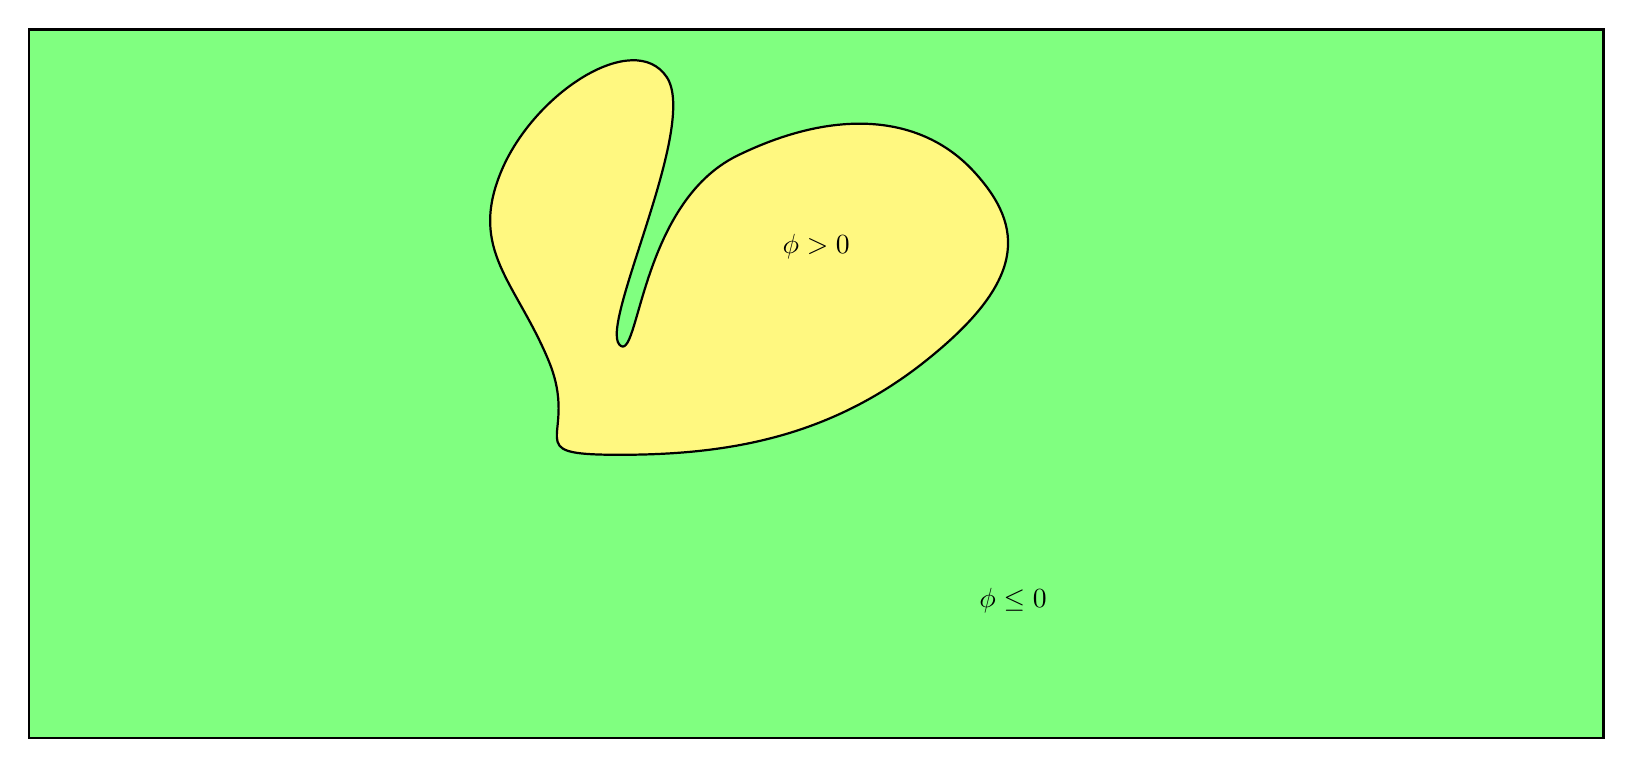
\begin{tikzpicture}[scale=2.5] % Adjust the outer scale factor to make the picture larger or smaller
			% Define the inner scale for the smooth region
			\def\innerScale{1.2} % Change this value to adjust the inner smooth region size
			
			% Draw rectangle with inner color
			\fill[green!50] (0, 0) rectangle (8, 3.6);
			\draw[thick] (0, 0) rectangle (8, 3.6);
			
			% Define the center and control points for the smooth region
			\begin{scope}
				\draw[thick, smooth, fill=yellow!50] 
				plot [smooth cycle, tension=1] coordinates {
					(3, 2) % Center point of the region
					(3 + 0.5*\innerScale, 2 + 0.8*\innerScale)
					(4 * \innerScale, 2.4 * \innerScale)
					(3.8 * \innerScale, 1.6 * \innerScale)
					(3, 1.2 * \innerScale)
					(2.2 * \innerScale, 1.6 * \innerScale)
					(2 * \innerScale, 2.4 * \innerScale)
					(2.7 * \innerScale, 2.8 * \innerScale)
				};
			\end{scope}
			
			% Labels for the rectangle and the region
			\node at (4, 2.5) {$\phi>0$};
			\node at (5, 0.7) {$\phi\leq0$};
			
		\end{tikzpicture}
		
		
		
		
	\end{multicols}
	
	
	
	\vspace{2cm} % Space between rows
	
	% Numerics row block with three horizontally aligned boxes
	\section*{Active Flux Method}
	
	\begin{multicols}{2} % Three columns for the three boxes
		% Box 1: Time Integration
		%		\begin{tcolorbox}[colback=green!5!white, colframe=green!75!black, title=Active FLux]


		
		\begin{tcolorbox}[colback=yellow!5!white, colframe=yellow!75!black, title=\textcolor{black}{\textbf{Sketch of control variables}}]
			

			\centering
			\begin{multicols}{2}

			\begin{minipage}[t][23cm][c]{0.8\textwidth}


			\vspace{3.cm}
			\begin{tikzpicture}[scale=4]
				\tikzset{dot/.style={fill=black,circle}}
				
				\draw [black] (0,1) -- (6.1,1);
				
				\draw (0.5,1) -- (0.5,1.7);
				\draw (1.5,1) -- (1.5,1.7);
				\draw (0.5,1.7) -- (1.5,1.7);
				\filldraw[blue] (1,1.7) circle (2pt);
				
				\draw (1.5,1) -- (1.5,2.7);
				\draw (2.5,1) -- (2.5,2.7);
				\draw (1.5,2.7) -- (2.5,2.7);
				\filldraw[blue] (2,2.7) circle (2pt);
				
				\draw (2.5,1) -- (2.5,3.7);
				\draw (3.5,1) -- (3.5,3.7);
				\draw (2.5,3.7) -- (3.5,3.7);
				\filldraw[blue] (3,3.7) circle (2pt);
				
				\draw (3.5,1) -- (3.5,3.2);
				\draw (4.5,1) -- (4.5,3.2);
				\draw (3.5,3.2) -- (4.5,3.2);
				\filldraw[blue] (4,3.2) circle (2pt);
				
				\draw (4.5,1) -- (4.5,2.2);
				\draw (5.5,1) -- (5.5,2.2);
				\draw (4.5,2.2) -- (5.5,2.2);
				\filldraw[blue] (5,2.2) circle (2pt);
				
				\foreach \x in {1.5,2.5,...,4.5}
				{
					\draw [dashed] (\x,0.5) -- (\x,4.5); %vertical lines at interfaces
				}
				
				\node at (2,0.6){$x_{i-1}$};
				\node at (3,0.6){$x_{i}$};
				\node at (4,0.6){$x_{i+1}$};
				
				\node at (1.5,0.35){$x_{i-\frac{3}{2}}$}; 
				\node at (2.5,0.35){$x_{i-\frac{1}{2}}$}; 
				\node at (3.5,0.35){$x_{i+\frac{1}{2}}$}; 
				\node at (4.5,0.35){$x_{i+\frac{3}{2}}$}; 
				
				\node at (1.5,4.7){$\textcolor{red}{\uvec{V}_{i-\frac{3}{2}}}$};
				\node at (2.5,4.7){$\textcolor{red}{\uvec{V}_{i-\frac{1}{2}}}$};
				\node at (3.5,4.7){$\textcolor{red}{\uvec{V}_{i+\frac{1}{2}}}$};
				\node at (4.5,4.7){$\textcolor{red}{\uvec{V}_{i+\frac{3}{2}}}$};
				
				\node at (1.5,5.2){$\textcolor{red}{\phi_{i-\frac{3}{2}}<0}$};
				\node at (2.5,5.2){$\textcolor{red}{\phi_{i-\frac{1}{2}}<0}$};
				\node at (3.5,5.2){$\textcolor{red}{\phi_{i+\frac{1}{2}}>0}$};
				\node at (4.5,5.2){$\textcolor{red}{\phi_{i+\frac{3}{2}}>0}$};    


				\node at (1.5,5.6){$\textcolor{black}{\gamma_2}$};
				\node at (2.5,5.6){$\textcolor{black}{\gamma_2}$};
				\node at (3.5,5.6){$\textcolor{black}{\gamma_1}$};
				\node at (4.5,5.6){$\textcolor{black}{\gamma_1}$};

				
				\node at (2,3){$\textcolor{blue}{\uvec{U}_{i-1}}$};
				\node at (3,4){$\textcolor{blue}{\uvec{U}_{i}}$};
				\node at (4,3.5){$\textcolor{blue}{\uvec{U}_{i+1}}$};
				
				% Drawing red crosses with adjustable size and thickness
				\foreach \x in {0.5,1.5,2.5,...,4.5,5.5}
				{
					\draw[red, line width=5.pt] (\x-0.1,1.3) -- (\x+0.1,1.5); % Diagonal line /
					\draw[red, line width=5.pt] (\x-0.1,1.5) -- (\x+0.1,1.3); % Diagonal line \
				}
				
			\end{tikzpicture}


			\vspace{2.cm}

				 

			\end{minipage}

%			\columnbreak


			\begin{minipage}[t][20cm][c]{0.33\textwidth}

				\centering

				
				
				Uniform mesh ($\Delta x$)		
				\begin{itemize}
					\item[$\textcolor{blue}{\bullet}$] $\textcolor{blue}{\uvec{U}_i}$ at \textcolor{blue}{cell centers}
					\item[$\textcolor{red}{\uvec{\times}}$] $\textcolor{red}{\uvec{V}_{i+\frac{1}{2}}}~\text{and}~\textcolor{red}{\phi_{i+\frac{1}{2}}}$~at~\textcolor{red}{cell~interfaces}
				\end{itemize}
				

			\end{minipage}


			\end{multicols}



		\end{tcolorbox}
		
		% Box 2: Spatial Discretization
		\begin{tcolorbox}[colback=yellow!5!white, colframe=yellow!75!black, title=\textcolor{black}{\textbf{Discretization}}]
			\centering
			\begin{itemize}
				\item Active flux discretization~[2,3,4]
			\end{itemize}
			
			\begin{align*}
				\begin{cases}
					\frac{d}{d t}\textcolor{blue}{\uvec{U}_i}(t)&=-\frac{\uvec{F}(\textcolor{red}{\uvec{V}_{i+\frac{1}{2}}})-\uvec{F}(\textcolor{red}{\uvec{V}_{i-\frac{1}{2}}})}{\Delta x}\\
					\frac{d}{d t}\textcolor{red}{\uvec{V}_{i+\frac{1}{2}}}(t)&\approx \textcolor{teal}{\left[-\frac{\partial}{\partial x}\uvec{\widetilde F}(\uvec{V})+\textcolor{violet}{\B(\uvec{V})\frac{\partial}{\partial x}\uvec{V}} \right]_{i+\frac{1}{2}}}\\
					\frac{d}{d t}\textcolor{red}{(\rho \phi)_{i+\frac{1}{2}}}(t)&\approx \textcolor{teal}{\left[-\frac{\partial}{\partial x}(\rho \phi v)\right]_{i+\frac{1}{2}}}\\
				\end{cases}
			\end{align*}
			
			\centering
			
			\begin{itemize}
				\item \textcolor{teal}{$2^{\text{nd}}$-order (PWL) \textcolor{violet}{PC}CU discretization}~[5]
				\item RK in time
				\item Cartesian setting dimension by dimension
				
			\end{itemize}
			
			\vspace{1.5em}
			
		\end{tcolorbox}



		
		% Box 3: Velocity Divergence
		\begin{tcolorbox}[colback=yellow!5!white, colframe=yellow!75!black, title=\textcolor{black}{\textbf{Conservative post--processing}}]
			
			\centering

			\vspace{1.5em}
			
			%					\centering
			\begin{itemize}
				\item \textcolor{blue}{Conserved variables} $\Rightarrow$ Correct solution
				\item \textcolor{red}{Primitive variables} $\Rightarrow$ \textcolor{violet}{Wrong solution}~[6]
			\end{itemize}

			PP to link evolution of the two variables
			
			\vspace{1.5em}
			
		\end{tcolorbox}
		
	\end{multicols}
	
	\vspace{2cm} % Space between rows
	
	% Results row block with two horizontally aligned boxes
	\section*{Numerical results}
	
	\begin{multicols}{3} % Two columns for the two boxes
		% Box 1: Shock Tube Test
		\begin{tcolorbox}[colback=red!5!white, colframe=red!75!black, title=\textcolor{black}{\textbf{Shock--bubble interaction}}]
			Bubble invested by a moving shock of air~[7]
			
			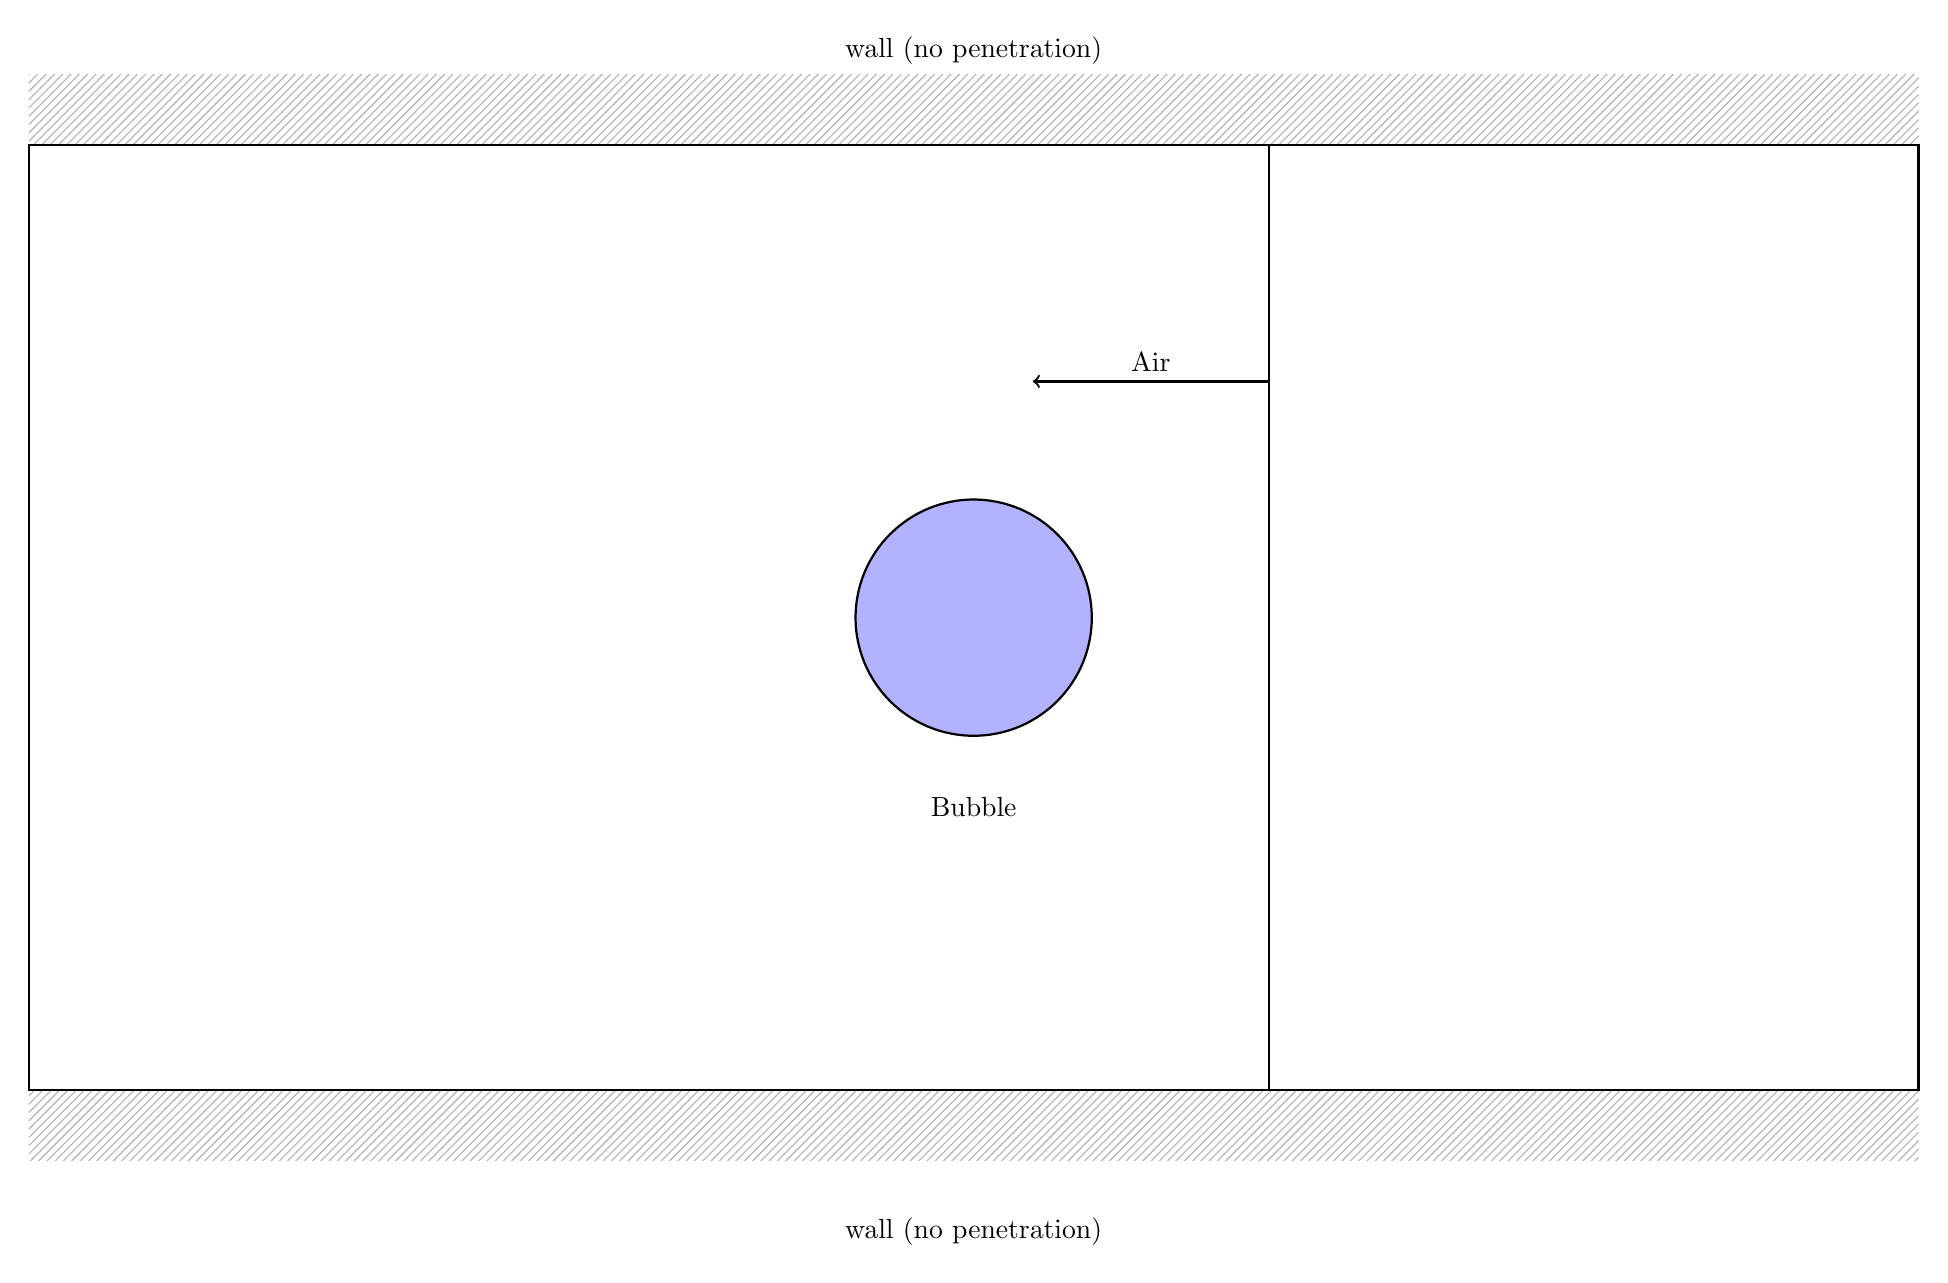
\begin{tikzpicture}[scale=3] % Adjust the scale factor to make the picture larger or smaller
				
				% Define the length of the walls
				\def\length{8} % Adjust this value for the wall length
				
				% Wall patterns
				\fill[pattern=north east lines, pattern color=black!30] 
				(-\length/2, 4) -- (\length/2, 4) -- (\length/2, 4.3) -- (-\length/2, 4.3) -- cycle;
				\fill[pattern=north east lines, pattern color=black!30] 
				(-\length/2, 0) -- (\length/2, 0) -- (\length/2, -0.3) -- (-\length/2, -0.3) -- cycle;
				
				% Draw rectangle, centered according to \length
				\draw[thick] (-\length/2, 0) rectangle (\length/2, 4);
				
				% Draw the bubble (circle) at the center
				\draw[thick, fill=blue!30] (0, 2) circle (0.5); % Circle representing the bubble
				
				% Draw the wave (vertical line) displaced to the right
				\draw[thick] (\length/2 - 2.75, 0) -- (\length/2 - 2.75, 4); % Vertical line representing the wave
				
				% Draw the arrow indicating wave movement towards the left
				\draw[->, thick] (\length/2 - 2.75, 3) -- (\length/2 - 3.75, 3) node[midway, above] {Air};
				
				% Labels for the bubble and wave
				\node at (0, 1.2) {Bubble};
				
				\node[above] at (0, 4.3) {wall (no penetration)};
				\node[below] at (0, -0.5) {wall (no penetration)};
				
			\end{tikzpicture}
		
			\centering
			\begin{itemize}
				\item Helium (left)
				\item R-22 (right)
			\end{itemize}
			
			
		\end{tcolorbox}
		
		
		
		
		
		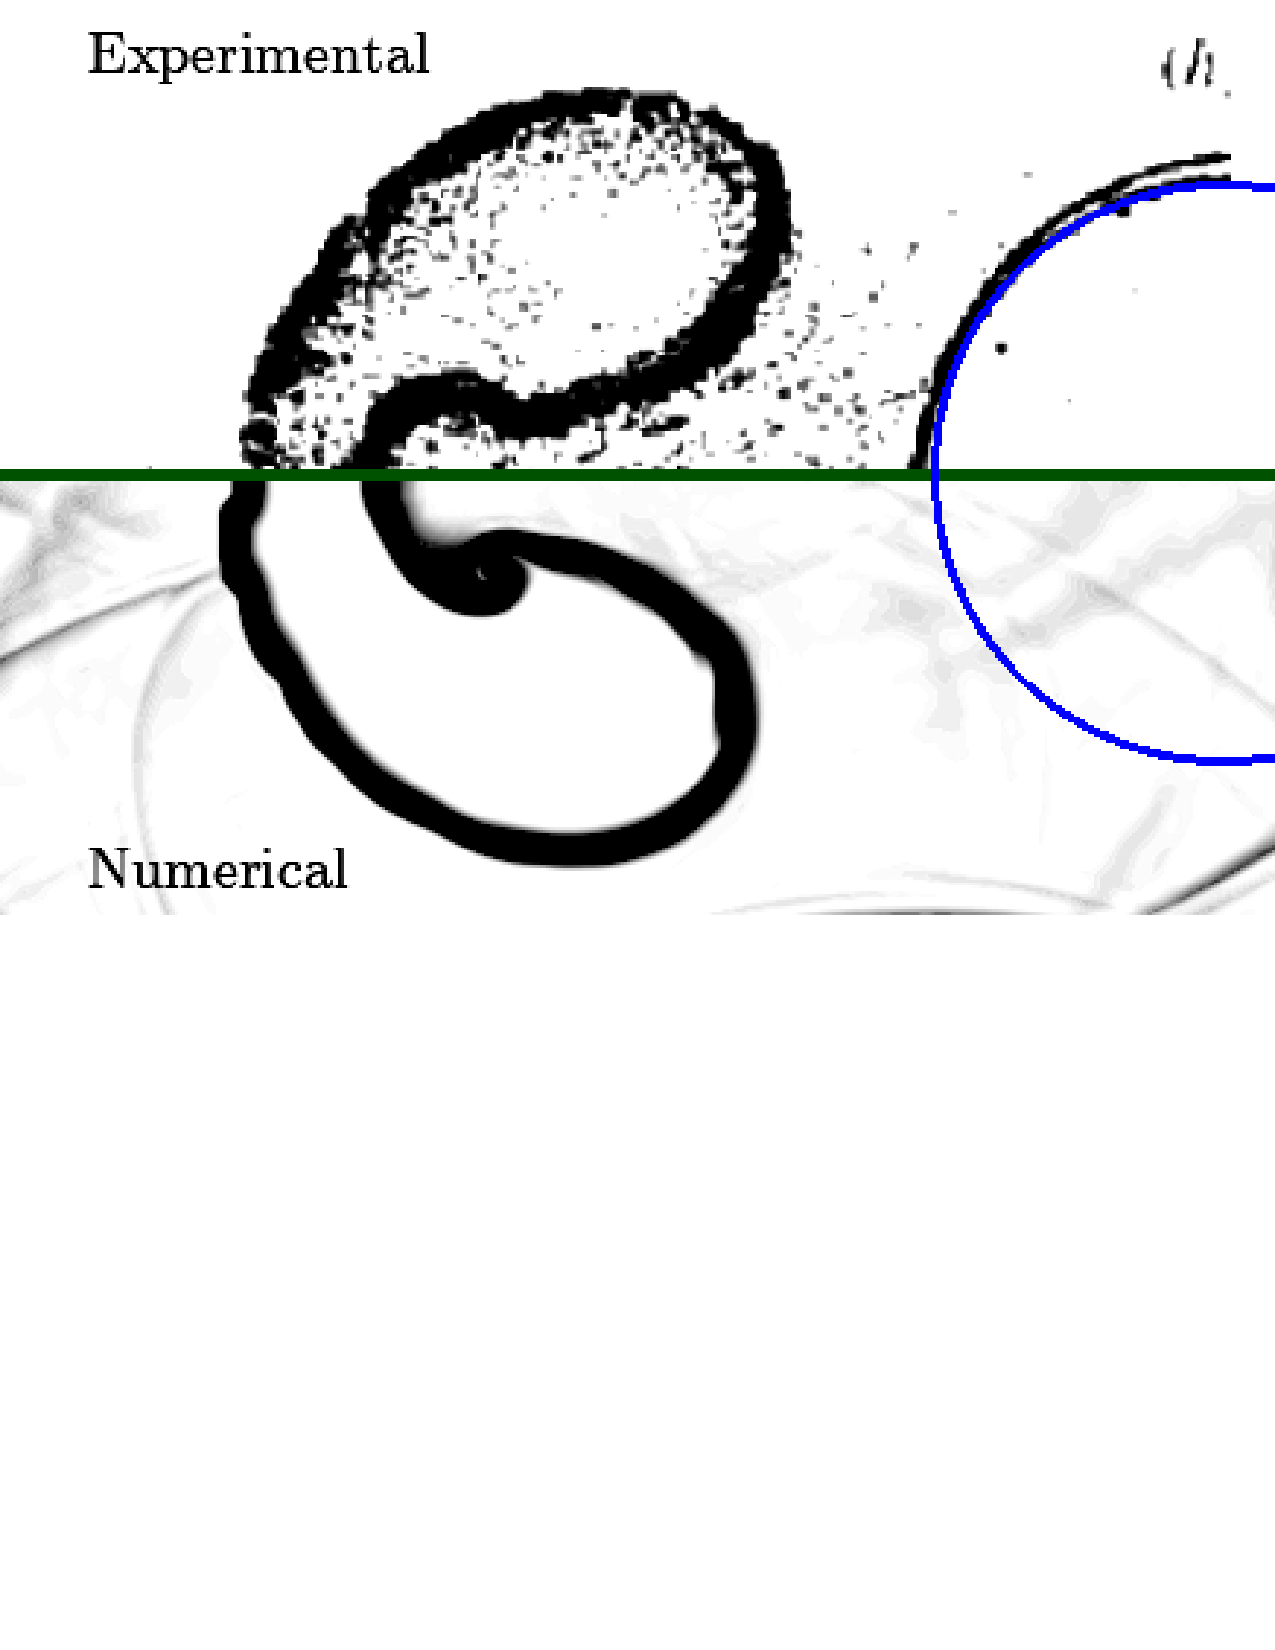
\includegraphics[width=0.9\linewidth]{results/helium_cropped.pdf} % Adjust the path and size
		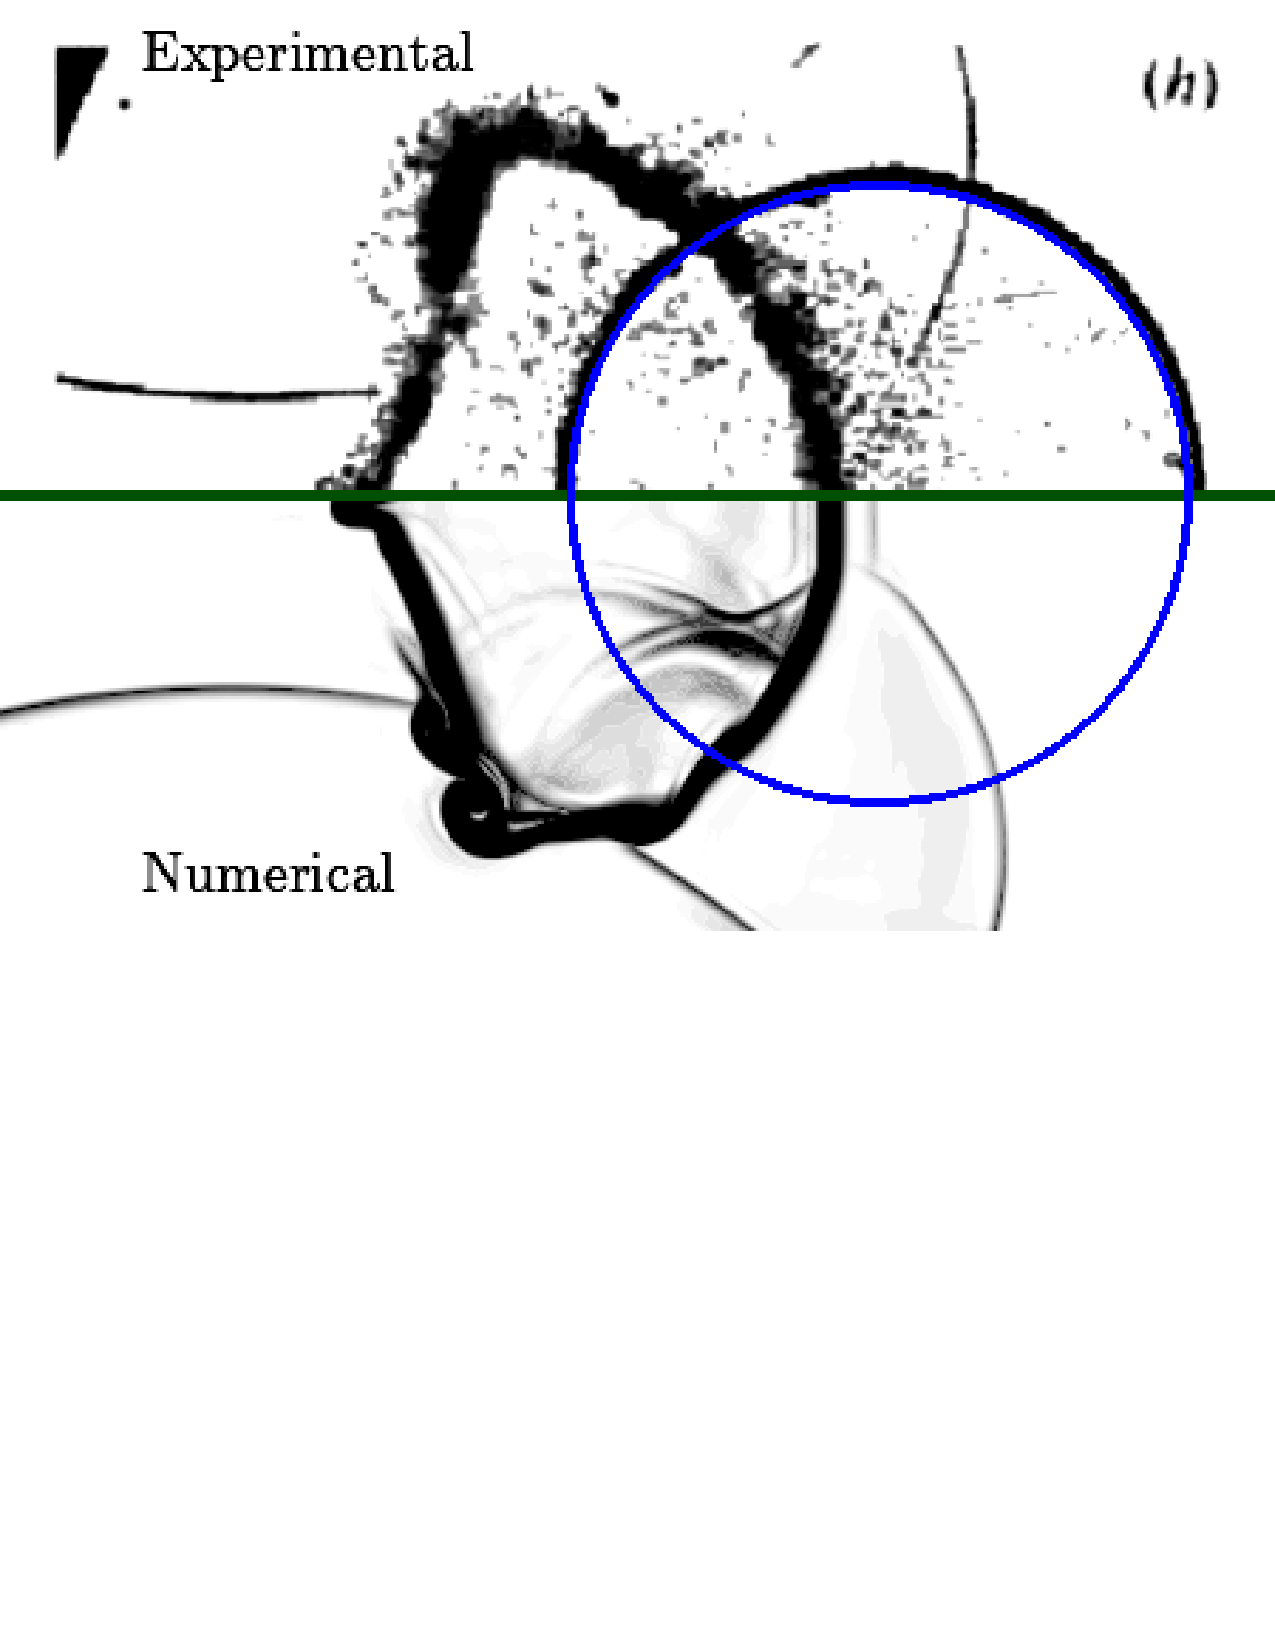
\includegraphics[width=0.9\linewidth]{results/r22_cropped.pdf} % Adjust the path and size
	\end{multicols}
	
	
	\vspace{-5.5cm}
	
	% References Section
	\section*{References}
{\Large % Change this to \large or \LARGE for different sizes
	\begin{itemize}
		\item~~[1] A. Chertock, S. Chu, A. Kurganov, 2021, Hybrid Multifluid Algorithms Based on the Path-Conservative Central-Upwind Scheme.
		\item~~[2] B. van Leer, 1977, Towards the ultimate conservative difference scheme. IV. A new approach to numerical convection.
		\item~~[3] T. A. Eymann, P. L. Roe, 2011, Multidimensional active flux schemes.
		\item~~[4] W. Barsukow, 2021, The active flux scheme for nonlinear problems.
		\item~~[5] M. J. C. Diaz, A. Kurganov, T. M. de Luna, 2019, Path-conservative central-upwind schemes for nonconservative hyperbolic systems.
		\item~~[6] R. Abgrall, S. Karni, 2010, A comment on the computation of non-conservative products.
		\item~~[7] J.-F. Haas, B. Sturtevant, 1987, Interaction of weak shock waves with cylindrical and spherical gas inhomogeneities.
	\end{itemize}
}

\end{document}

